\chapter{Discussion}
\label{cha:discussion}

In this chapter we briefly summarize the findings from the previous 3 chapters regarding the needs of forced migrants in Münster, the design of solutions that meet those needs, and the usefulness and usability of the designs that we created. We then discuss these findings in a wider context and clarify the limitations of this work.


\section{Discussion of Needs}

We identified 55 forced migrant needs in regards to reducing social isolation. Here we discuss five key needs which we tried to address with the prototype that we developed.

\subsubsection*{Contact with a local ``introducer''}

Similar to the findings of \citeA[p. 5]{schreieck_supporting_2017} that a ``local contact person'' is the most important source of information for newcomers, we found that meeting an ``introducer'' is their most important source of social connection.

All of the forced migrants with whom we talked explained the importance of meeting a local with a strong social network who is able to introduce newcomers to potential new contacts. Most described just one key person who had introduced them to many friends.

\subsubsection*{Home where contact can be developed}

Forced migrants commonly invite people into their homes as a strategy to make meaningful social contacts. All of our participants mentioned using this strategy at least once. To do this, however, forced migrants must have a home that can accommodate guests. They must be able to communicate their home's location to others and feel confident and safe doing so.

\subsubsection*{Accommodation of low language abilities}

Perhaps the most discussed topic in our interviews about making social contact in Münster was the challenge of connecting with people without knowing much German. All of our participants experienced and overcame this challenge. They highlighted the need both for translators and translated resources when forced migrants first arrive, but also for opportunities to learn the local language.

\subsubsection*{Basis to initiate contact}

A commonly known strategy for making social contacts, not just among forced migrants but also in many other circles of society, is to seek out people with common interests. All of our participants reported doing this. They explained commonalities provide a basis to initiate a first conversation and an excuse to meet up again.

\subsubsection*{Element of spontaneity and scheduling flexibility}

Newcomers have busy, shifting, and complex schedules due to the wide variety and irregularity of important tasks they must complete in order to settle into their new home \cite[p. 17]{bustamante_duarte_exploring_2018}. We heard repeatedly that in order to make social contacts, one must find opportunities that fit with one's schedule. Often this means being spontaneous and approaching strangers to join a football match, start a conversation in a public place, or to offer help.

% \subsubsection*{Opportunity to express oneself}
% \subsubsection*{Open and safe social opportunities}
% \subsubsection*{Opportunity to learn}
% \subsubsection*{Sense of help}

% \subsection*{Overlap of Needs}
% \label{sec:overlap_of_needs}


\section{Discussion of Designs}
\label{sec:features}

\subsection*{Overview}

We came up with a number of design solutions to meet the above needs with features of a location-based freecycling service. We did this by implementing a subset of the user requirements developed during the needs assessment phase.

\subsection*{Selected Features}

Following is a list of some of the more interesting features we implemented. For each feature we describe why we found the feature was important for a location-based freecycling service to reduce social isolation and why we implemented it the way we did.

\subsubsection*{Authentication}

Authentication is essential in any system where it is important to know that users are who they say they are. When freecycling, you have to know the person you are contacting is actually the person who posted the offer in which you are interested. When there is the potential to meet up in person, it becomes even more important that the identity of the users is somehow validated.

We decided to use passwordless authentication to make it easy to sign up and sign in. During the needs assessment we heard that many in our user groups had no desire to create another account and remember yet another password. We chose to allow people to sign in with Facebook and Google because 1) Facebook is the primary platform for freecycling in Münster, meaning most freecyclers are already connected and familiar with it, and 2) among our participants, Facebook and Google/Gmail/YouTube were the two most commonly referenced digital services after WhatsApp, which doesn't provide its own authentication service.

We decided to additionally give users the option to sign up with their email and a secure password. While having to enter these details is usually less convenient, several participants from our needs assessment study expressed a preference for services that did not require connection with large corporate social networks like Facebook. Providing this third option allowed users to make the choice themselves between convenience and anonymity.

\subsubsection*{User approval}

Approving new users was identified as the primary task of freecycling moderators. Local freecyclers repeatedly mentioned feeling reassured about the trustworthiness of other users because of the approval process. We also learned that forced migrants have their own system for approving new social contacts, often employing the very same strategies as freecycling moderators. These strategies include asking simple questions to see if the other could provide ``normal'' responses, identifying if the other is a part of a group that the approver trusts, and keeping an eye out for conflicting political beliefs.

User approval serves as an obstacle to spam bots or their social equivalent: people who make new contacts in order to broadcast a message or achieve some financial gain. It also contributes to community safety by prohibiting users with obvious malicious intent from accessing the data of other users.

The downside of user approval is that it makes the service exclusive and requires someone to judge potential new members, which is nearly impossible to do impartially. In fact, moderators indicated that this may be one reason why forced migrants are not well represented in freecycling groups in Münster: when a new user's profile is in another language and does not show signs of already being part of trusted Münster communities, the moderator is likely to reject the membership request.

We implemented approval as a simple boolean attribute on the user object. In the absence of a moderator user interface, the attribute can only be updated via direct access to the database. After signing up, new users are redirected to a screen informing them that they will receive an email when their account is approved.

Location-based services enable an additional means of approval. In the Geofreebie prototype, users are automatically approved to make an offer available based on their physical presence in Münster. A bounding box geofence surrounds the city limits and users outside of this fence are automatically shown as ``unavailable'' in the system. This reduces misuse of the system by filtering out users actually located in other cities, which is a common concern among freecycling moderators.

\subsubsection*{In-app forms}

We chose to implement the study consent form and study surveys as in-app forms for a number of reasons. This allowed us to require users to fill out certain forms before using the system, ensuring that consent was timely. This also allowed us to recruit participants without meeting them in person, as no physical paperwork was required to participate in the study.

We implemented the consent form as a page of explanatory text followed by four check boxes and a submit button. We chose this design in order to mimic the paper consent form of our institution. At the top of the consent screen, the user can select the language of the form. This allows users to see the information in multiple languages, which can improve comprehension.

We also require users to fill out two surveys before using the app. Chapter~\ref{cha:evaluation} describes the surveys and their purpose within the third phase of the study. These questionnaires are mostly multiple-choice questions, for which we use radio buttons because they are more usable than dropdown menus in a mobile app context. There is also one question about where the participant grew up, which we implemented as a free-text input to allow flexibility in the response. Again, each form is validated for completeness when the user tries to submit it, and access to the app is not allowed until the user completes the questionnaires.

\subsubsection*{User communication}

Communication is an equally essential part of freecycling and making social contacts in a new city. People have a wide variety of preferences and strategies when it comes to how they communicate. Therefore, we decided to give users a number of communication options to suit their personal preferences.

We designed interactions such that the person making the offer gets to choose the method of communication. This was reported to be common practice on Münster's Facebook-based freecycling platforms, where users would often state if they preferred to be contacted via comment or private message.

Users choose how others can contact them on the settings page (see figure~\ref{fig:scr_settings}). Toggle switches control their response to the question ``How do you want to be contacted?'' and when a certain contact mode is enabled, a text field appears where the contact details for that mode can be entered.

\begin{figure}[ht]
  \centering
  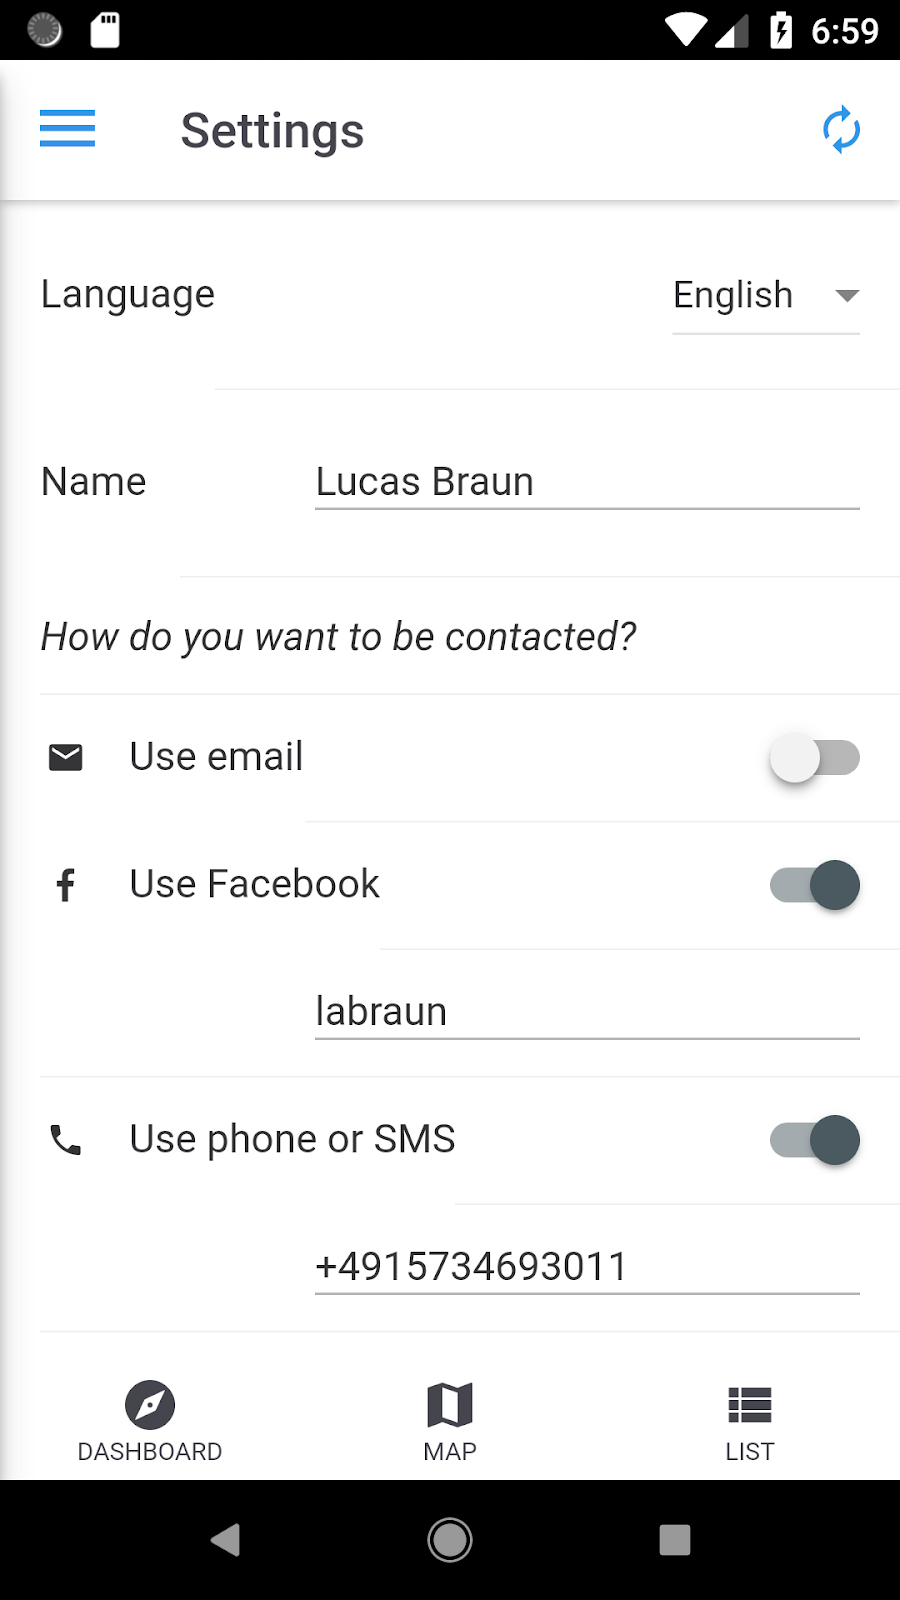
\includegraphics[scale=0.25]{images/screenshots/screenshot_settings.png}
  \caption{Prototype settings page}
  \label{fig:scr_settings}
\end{figure}

The four contact options we provided were email, Facebook, phone, and WhatsApp. These were the four most popular communication methods of the participants in our needs assessment study, matching the findings of \citeA{xu_communication_2016}.

After a user provides contact details, links are automatically generated from this information for other users to click on. Phone links and email links are a standard part of modern HTML (see the first two examples in table~\ref{tab:contact_link_examples}). They provide a way to launch communication in the context of a particular phone number or email address in the default phone or email application of the device on which the link is clicked. At the time of this writing, Facebook and WhatsApp provide a service to enable similar links for their services (see the last two examples in table~\ref{tab:contact_link_examples}). We made use of these links to seamlessly integrate other communication services into our freecycling service. Figure~\ref{fig:scr_map} shows an example of how these links appeared in the map view.

\begin{table}[ht]
\centering
\begin{tabular}{|l|l|}
\hline
\rowcolor{lightgray}
\textbf{Action}         & \textbf{Link Format}                                      \\ \hline
Open Phone or SMS       & \texttt{tel:\textless{}phone\_number\textgreater{}}       \\ \hline
Open Email              & \texttt{mailto:\textless{}email\_address\textgreater{}}   \\ \hline
Open WhatsApp           & \texttt{wa.me/\textless{}phone\_number\textgreater{}}     \\ \hline
Open Facebook Messenger & \texttt{m.me/\textless{}facebook\_username\textgreater{}} \\ \hline
\end{tabular}
\caption{Contact link formats}
\label{tab:contact_link_examples}
\end{table}


\subsubsection*{Language and localization}

We decided to make the app available in several languages in order to meet the need for accessibility to those with low German abilities. We implemented a language-switching feature called the locale menu, which is present in a number of places around the app (see figure~\ref{fig:scr_locales}).

We implemented the translation of the app's strings in one file: \textit{localizations.json}. This made it simple for more languages to be added: a volunteer translator simply needed to go through and translate the list of 180 short strings, which usually took less than one hour, and then the new strings could be copied and pasted into a new element in the JSON array of localizations. By the time the trial had begun, the app had been translated from English into German, Arabic, Nepali, and Spanish. During the trial, another volunteer stepped forward to help with Amharic, and a Farsi native speaker expressed interest as well.

The fact that the language menu is prominently present in several places (e.g., the help pages, the consent form, the settings page) and not just tucked away between other user preferences, is meant to accommodate those with low ability in one language while still encouraging them to learn other languages.


\begin{figure}[ht]
  \centering
  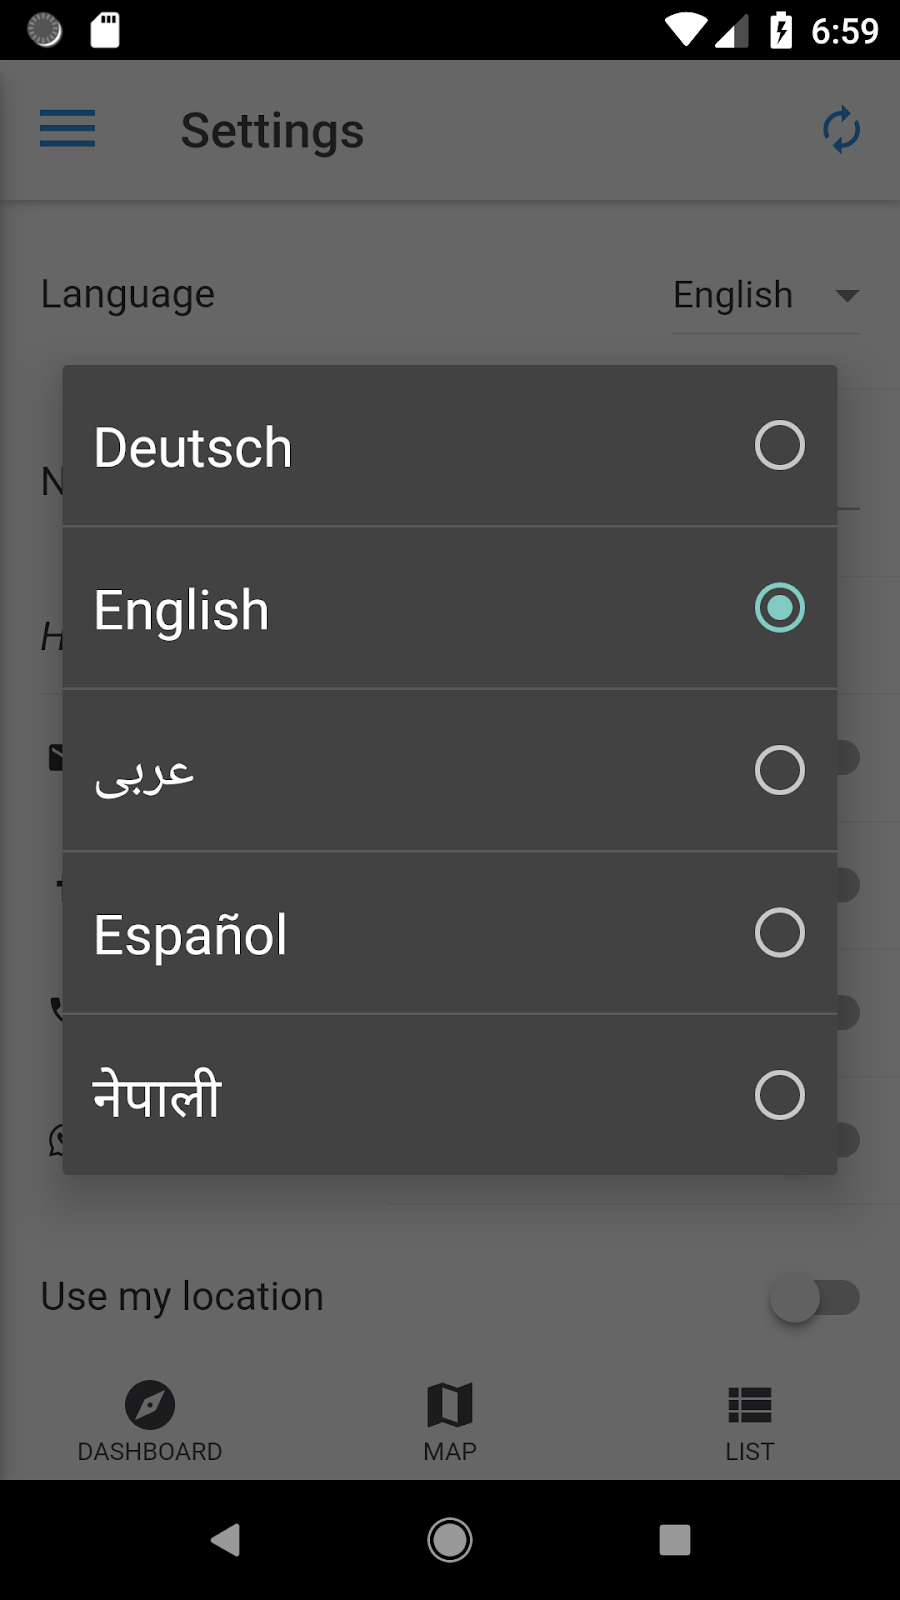
\includegraphics[scale=0.25]{images/screenshots/screenshot_locales.png}
  \caption{Prototype locale settings}
  \label{fig:scr_locales}
\end{figure}

\subsubsection*{Map and list views}

The map and list views of the prototype were intended to meet several needs at once (see figure~\ref{fig:scr_map}). The location-based features showing the distance to other users provides a basis to initiate contact (physical proximity) and facilitate those with limited language abilities to better visualize the offer and its location in the city. The Geofreebie star under the name of the person making the offer highlights the number of offers the user has already successfully delivered, thus indicating their status in the social network of the service and suggesting their potential as an ``introducer''. The app itself is also intended to play the role of the introducer by presenting potential contacts and suggesting reasons to connect.

\begin{figure}[ht]
  \centering
  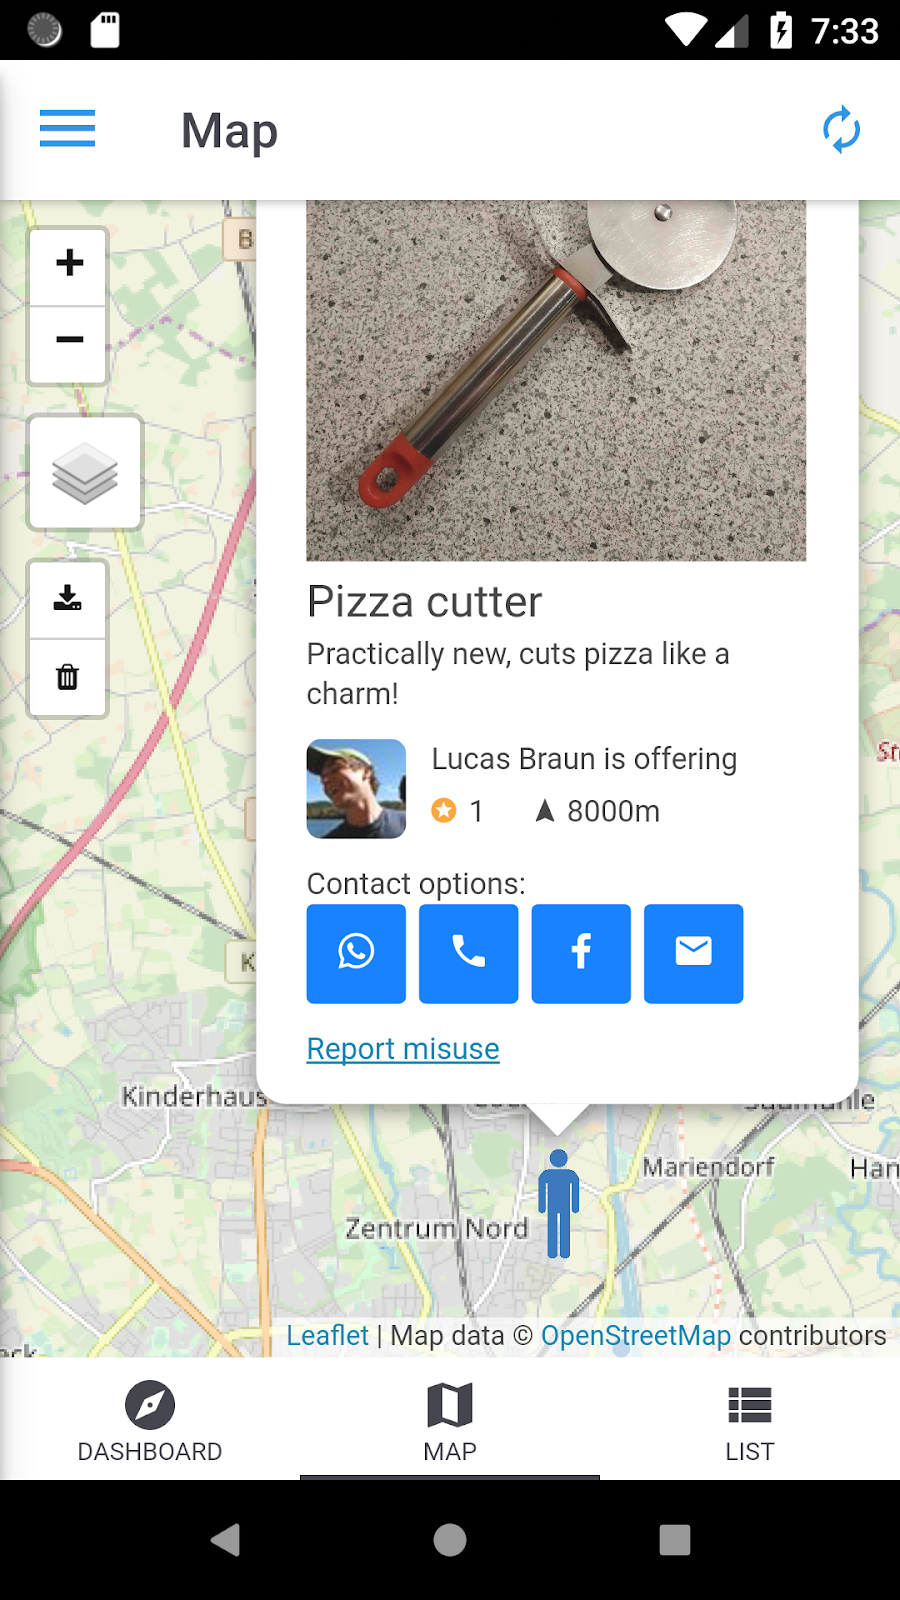
\includegraphics[scale=0.25]{images/screenshots/screenshot_map.png}
  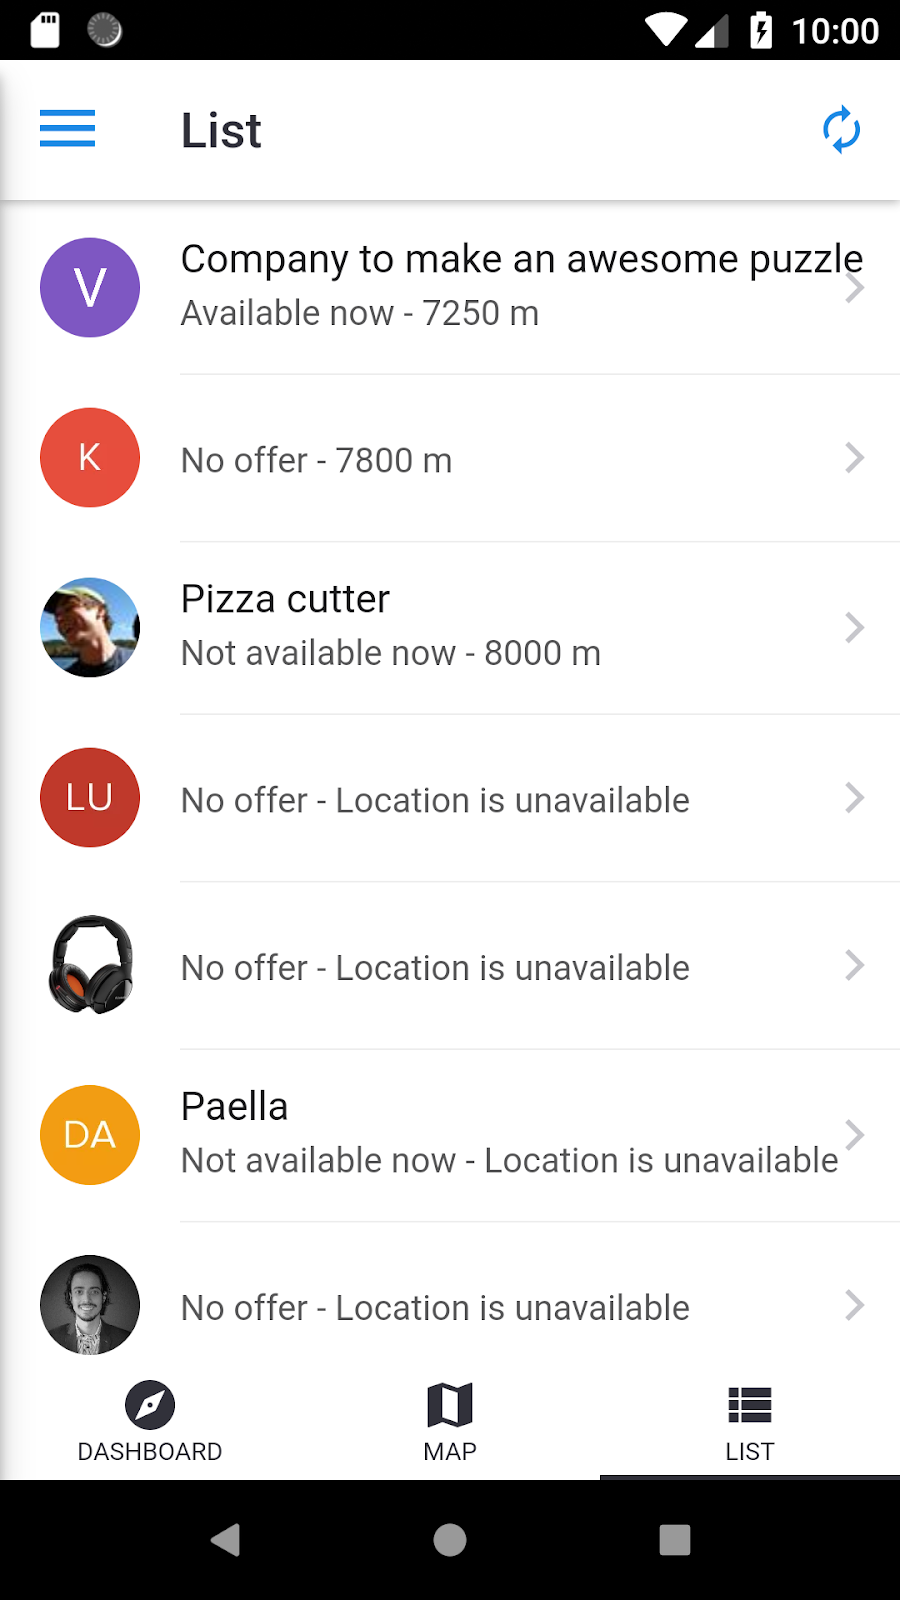
\includegraphics[scale=0.25]{images/screenshots/screenshot_list.png}
  \caption{Prototype map and list views}
  \label{fig:scr_list}
  \label{fig:scr_map}
\end{figure}

% \subsubsection*{Dashboard}
% \subsubsection*{Reviews}
% \subsubsection*{Authentication}
% \subsubsection*{Location settings}
% \subsubsection*{Offer completion}
% \subsubsection*{Navigation}

\subsubsection*{Help}

Offering help and technical support is important in any digital service. In digital services for vulnerable populations, we found it becomes especially important. These services must not only explain the functionality of the app but also address concerns about safety and privacy, all in a way that is easily understandable by users with a diversity of language abilities. Our help page includes five sections: help, rules, contact, privacy, and consent.

% \subsubsection*{Report link}

% See figure~\ref{fig:scr_map} for an example.

\subsubsection*{Back button}

One major cause of distress during pilot testing of the prototype was the back-button functionality on Android phones. Users are accustomed to being taken backwards one screen when they tap the back button, yet the default behavior in cordova apps is to exit the application entirely. This was quite frustrating to testers who were trying to reverse a mistaken navigation action, and instead got booted out of the system completely.

While not a revolutionary observation, the importance of respecting user expectations about basic UI functions is not to be overlooked. We updated the back button functionality to keep users in the app.

\subsubsection*{Reload button}

Pilot testing also revealed the need for a refresh button. Mobile users often do not trust their network connection and want to be sure that they have the latest version of shared data. Such a button gives them control to see the latest data when they want it, not at the standard interval when the app refreshes data automatically. We added a refresh button to the top right corner in the navigation bar, as can be seen in figure~\ref{fig:scr_map}.


\section{Discussion of Evaluation}

\subsection*{Usability}

A SUS score of 82 falls into the top quartile of the 206 studies analyzed in one meta study about SUS scores, and correlates with an adjective rating of ``excellent'' \cite{bangor_empirical_2008}. Although a high SUS score does not guarantee acceptability in the field, it does suggest promise and a lack of major usability issues.

More interestingly, both user groups gave close to the same average SUS score. This suggests that we successfully tailored the design solutions to both user groups through the human-centered design process.

% TODO: reference the Moin app findings

\subsection*{Potential Usefulness}

Our initial two-week trial of the prototype was not long enough to evaluate the full usefulness of the service. The relatively short duration of the trial was limiting for three reasons. First, building up a large user community takes time. Freecycling systems work best when there are a lot of users. The more users that are actively posting and browsing for offers, the higher the chance that someone will offer something that another user actually needs.

Second, as we identified in our needs assessment, both freecycling and making social contacts as a newcomer require good luck and patience. The longer someone is a member of a freecycling system, the more likely they are to find something they would like to offer or see an offer of interest.

Third, building relationships takes time. Even when people contact someone through a freecycling service, it takes time to arrange an in-person meetup. If this meetup is the first of repeated meetups, it may be a week or more before the next meetup takes place. In our model where the system is the ``introducer,'' extra time is also required for the users to build a relationship of trust with the system.

For these reasons we could only evaluate the potential of the prototype system for creating social contacts. The in-app sampling results showed high feasibility and success compared to other freecycling systems. The results of the usefulness survey were also promising. Here we discuss these results in terms of their potential.



\subsubsection*{Creation of new instances of social contact}

One participant reported having made a new social contact because of the app and described the interaction as positive and potentially leading to future repeat interactions. While this single result is not a significant indicator of the service's overall value in regards to generating new social contact between strangers, it does show the potential and feasibility of the idea.

Participants' generally disagreed with the statements ``I think using this system increased my contact with others during the last two weeks,'' ``I made contact with people outside of my normal circles through this system,'' and ``I think this app increased the size of my social network in Münster'' because they did not successfully complete any freecycling exchanges. Half of the forced migrants did think that the app increased the size of their social network, however. This may be due to the modern understanding that a social network can also be virtual. For this reason, we recommend that future services do more to foster this virtual community. One limitation of the prototype, for example, was that participants' contact information only became visible when they had posted an offer. Users should have the possibility to make themselves open to contact even if they do not have something to offer in the moment.
% Design recommendation

\subsubsection*{Creation of a trusting community}

Participants' general agreement with the statements ``I feel like part of a community while using this system'' and ``I think the contacts made through this app are likely to lead to new friendships'' also shows potential for reducing social isolation. Furthermore, only one participant disagreed with the statement ``I think I can trust the other users of this system.'' Feeling like part of a community, optimism about making new friendships, and contact with trustworthy people are all indicators of low social isolation \cite{cornwell_measuring_2009}.

% \subsection*{Design recommendations}

% \begin{itemize}
% \item Crowd sourced localization
% \item Contact options and HTML contact links
% \item Two-sided image formatting strategy
% \item In-app forms
% \item Diverse authentication options
% \end{itemize}


\section{Limitations}

There are several limitations to the results of this study. The number of participants and duration of the evaluation did not allow for a full assessment of the usefulness of the prototype service.

Furthermore, our recruitment strategies were biased towards forced migrant participants who were already social enough to be out meeting strangers, meaning less social people were underrepresented. Women and older forced migrants were also underrepresented, so our results may not fully reflect their needs and contexts.

Another limitation is our assumption that contact through a freecycling service does indeed reduce social isolation. Meeting another individual in person does not guarantee a positive social interaction.

% Bias of agree/disagree questions
